\published{IEEE Geoscience and Remote Sensing Letters, 12,  no. 11, 2316-2320 (2015)}

\title{Ground-roll noise attenuation using a simple and effective approach based on local bandlimited orthogonalization}
\renewcommand{\thefootnote}{\fnsymbol{footnote}}
\author{Yangkang Chen$^1$, Shebao Jiao$^2$, Jianwei Ma$^3$, Hanming Chen$^2$, Yatong Zhou$^4$, and Shuwei Gan$^2$}

\address{$^1$ Jackson School of Geosciences,
The University of Texas at Austin,
University Station, Box X,
Austin, TX 78713-8924, USA,
Email: ykchen@utexas.edu \\
$^2$ State Key Laboratory of Petroleum Resources and Prospecting, 
China University of Petroleum, 
Fuxue Road 18th,
Beijing, China, 102200, 
Email: gsw19900128@126.com \& huichanming@126.com \\
$^3$ Department of Mathematics,
Harbin Institute of Technology,
Harbin, China, 
jma@hit.edu.cn \\
$^4$ School of Electronic and Information Engineering,
Hebei University of Technology,
Xiping Road No. 5340, Beichen District,
Tianjin, China, 300401,
zyt@hebut.edu.cn 
}

\maketitle
%512375919@qq.com

%%%%%%%%%%%%%%%%%%%%%%%%%%%%%%%%%%%%%%%%%%%%%%
%	Defined by myself 
%%%%%%%%%%%%%%%%%%%%%%%%%%%%%%%%%%%%%%%%%%%%%%  
\newcommand{\dlo}[1]{}
\newcommand{\wen}[1]{#1}    

%%%%%%%%%%%%%%%%%%%%%%%%%%%%%%%%%%%%%%%%%%%%%%
%	Defined by myself 
%%%%%%%%%%%%%%%%%%%%%%%%%%%%%%%%%%%%%%%%%%%%%%

\begin{abstract}
% The bandpass filtering is a common way for estimating the ground-roll noise in land seismic data because of the low-frequency property of ground-roll noise. However, the frequency-overlap problem makes bandpass filtering inconvenient or even impossible to achieve a successful removal of ground-roll noise.  In this paper, we propose a novel band-limited orthogonalization approach for removing ground-roll noise without harming useful primary reflections. We orthogonalize the initially denoised signal via bandpass filtering with a relatively high low-bound-frequency (LBF), and the corresponding noise section that contains loss of primary reflections, using local signal-and-noise orthogonalization.  The local orthogonalization guarantees that the least coherent primary reflections are lost in the noise section. The procedure of the proposed approach is very convenient to implement because only a bandpass filtering and a regularized division between the initially denoised signal and initial noise are used. An open-source field dataset demonstrates a successful performance using the proposed approach. 
Bandpass filtering is a common way to estimate ground-roll noise on land seismic data, because of the relatively low frequency content of ground-roll. However, there is usually a frequency overlap between ground-roll and the desired seismic reflections that prevents bandpass filtering alone from effectively removing ground-roll without also harming the desired reflections. We apply a bandpass filter with a relatively high upper bound to provide an initial, imperfect separation of ground-roll and reflection signal. We then apply a technique called 'local orthogonalization' to improve the separation. The procedure is easily implemented, since it involves only bandpass filtering and a regularized division of the initial signal and noise estimates. We demonstrate the effectiveness of the method on an open-source set of field data.
\end{abstract}

%\begin{keywords}
%Ground-roll noise, bandpass filtering, local orthogonalization, regularized division
%\end{keywords}

\section{Introduction} 
Ground-roll noise is a type of coherent seismic noise, with a high amplitude, low frequency, and low velocity. It is often the strongest mode of coherent noise for land seismic surveys. Ocean bottom node (OBN) based marine seismic surveys may also contain this type of noise \cite{yangkang20142}. Ground-roll noise is a type of source-generated noise and can be scattered by near-surface heterogeneities.  The ground-roll noise often masks the shallow reflections at short offset, and deep reflections at larger offset \cite{claerbout1983,saatilar1988,henley2003}, and must be removed before the subsequent processing tasks. Instead of being incoherent along the spatial direction like random noise \cite{wencheng2015asa,yangkang2015}, the ground-roll noise is usually coherent along the spatial dimension, which can assist in its removal using simple signal processing methods.  There has been a lot of research about removing ground-roll noise published in the literature, and many researchers have proposed different methods for handling the ground-roll noise problem \cite{shieh1990,brown2000}. Most of the ground-roll noise removal approaches either fail to remove all the ground-roll noise or remove much useful primary reflection energy. An efficient and effective technique for removing ground-roll noise is always in demand. 

The simplest and most straightforward way for removing ground-roll noise might be bandpass filtering. Because of the low-frequency property of ground-roll, a simple high-pass filter is often applied to the seismic record to attenuate the ground-roll noise. However, the low-bound-frequency (LBF) for the bandpass filter is not easy to choose, because higher LBF will damage primary reflections while lower LBF will fail to remove enough ground-roll noise. This issue exists because of the frequency overlap of primary reflections and ground-roll noise. One way to solve this problem is to use matched filtering. The low-pass data is used as an initial guess for the ground-roll noise and then a least squares (LS) based matching filter is calculated to match the initial ground-roll noise to the raw seismic data best \cite{carson2006,stephen2007,halliday2010}. The matched ground-roll noise is then subtracted from raw seismic data to obtain the output. This adaptive subtraction method depends highly on the initial prediction of the ground-roll noise. Besides, in the case of highly non-stationary primary reflections and ground-roll noise, a conventional stationary matched filtering will fail to obtain an acceptable result.  

%\cite{james1968} proposed the multichannel stacking filters for attenuating those types of noise which \dlo{occur}\wen{occurred} at relatively well-determined points on neighbor traces, such as the ground-roll noise. \cite{prasad1980} studied and compared the performance of the least-mean-squares (LMS) adaptive filter, the adaptive lattice filter, and the adaptive Kalman filter identifier.  \cite{cahit1983} proposed an effective surface wave removal approach termed as vibroseis whitening (VSW) approach, which was tailed specifically for vibroseis data. The VSW approach was based on the application of time-varying amplitude scaling before vibroseis crosscorrelation. This scaling resulted in a signal-to-noise ratio (SNR) improvement equal\dlo{s} to the gain expected from crosscorrelation. This approach \dlo{is}\wen{was} also termed as the spectral balancing approach. \cite{ruhi1988} proposed a one-dimensional, linear frequency-modulated matched filter for removing ground-roll noise. This approach works well when the frequency bands of seismic reflections and ground-roll noise overlap. \cite{carson2006} proposed to use curvelet transform to remove ground-roll noise by a two-step process. The first step is to identify the ground-roll noise from the seismic data using an appropriate approach and then separate the signal and ground-roll noise using a block-coordinate relaxation method that seeks the sparest set for weighted curvelet coefficients of the ground-roll noise and the sought-after reflectivity. \cite{ruhi1994} proposed an adaptive lattice filter for attenuating ground-roll noise. The lattice filter has the same order of computational complexity as the LMS adaptive filter but enjoys a faster convergence rate.  \wen{\cite{regone1998} and \cite{ozbek2000} proposed to use acquisition-based suppression schemes to attenuate the ground-roll noise based on the use of recording arrays. \cite{stephen2007} proposed a polarization filtering approach to attenuate ground-roll noise, in which they combined statics, signal-to-noise ratio, and eigenimages to construct the ground-roll noise model, followed by adaptive subtraction.}  \wen{There is a type of ground-roll noise attenuation approaches that are based on the seismic interferometry \cite{halliday20072,halliday20092}.} \cite{yanwei2009} proposed an interferometric method to predict and subtract surface waves in seismic data. Instead of the traditional frequency-based one-step prediction, the interferometric method uses a multi-prediction and subtraction strategy to attenuate more ground-roll noise and preserve more useful energy. However, the implementation requires a careful parameters designing and tuning process. \wen{\cite{halliday2010} also proposed an interferometric ground-roll removal approach. They used seismic interferometry to estimate scattered ground-roll noise between pairs of receiver locations.}   A recently proposed approach by \cite{liuyang2012} utilized a time-frequency decomposition technique to separate ground-roll noise and primary reflections. The basic principle of this method is that instead of using a global frequency difference between the primary reflections and ground-roll noise, it uses the local time-frequency property of ground-roll noise to achieve the noise free data. 
In this paper, we proposed a simple but effective way for removing all the ground-roll noise without harming useful reflections. We first apply a simple bandpass filter to raw seismic data in order to remove all the ground-roll noise (thus the LBF should be a little bit high to guarantee no ground-roll noise left in the data). Then because of loss of useful primary reflections, we use local signal-and-noise orthogonalization proposed recently by \cite{yangkang2015ortho} to orthogonalize the primary reflections and ground-roll noise in order to restore the lost useful signals to the initial bandpass filtered data. The local orthogonalization algorithm was initially proposed to compensate for the useful energy loss during a traditional random noise attenuation process. The basic principle of the local orthogonalization methodology is to assume that the useful signal and noise should be orthogonal to each other and then orthogonalize the two components by formulating a regularized inverse problem. We bring the same strategy to this paper to compensate for the energy loss in a simple bandpass filtering based ground-roll noise attenuation approach. The performance of the proposed approach on the pre-stack dataset appears successful and also indicate a broader application of the orthogonalization methodology in removing various types of noise.    

\section{Method}
\subsection{Bandpass filtering and the frequency-overlap problem}
A bandpass filtering process can be simply summarized as:
\begin{equation}
\label{eq:bandpass}
\mathbf{\hat{d}} = \mathbf{F}^{-1} \mathbf{B}_{fl,fh} \left(\mathbf{F} \mathbf{d}\right),
\end{equation}
where $\mathbf{d}$ and $\mathbf{\hat{d}}$ denote the unfiltered and filtered data, respectively. $\mathbf{F}$  and $\mathbf{F}^{-1}$ denotes a pair of forward and inverse Fourier transforms. $\mathbf{B}_{fl,fh}$ denotes the bandpass filter with a high-bound-frequency (HBF) $fh$, and low-bound-frequency (LBF) $fl$. For the purpose of removing ground-roll noise, $fh$ is usually chosen as Nyquist frequency, the only parameter to choose is the LBF. The actual filtering in this paper is implemented by recursive  (Infinite Impulse Response) convolution in the time domain following the Butterworth algorithm.

The problem of bandpass filtering for removing ground-roll noise is the difficulty of choosing an optimal LBF, because of the frequency-overlap problem of ground-roll noise and primary reflections. Figure \ref{fig:field-1-0,dif-1-0,field-2-0,dif-2-0} shows a demonstration of the frequency-overlap problem. When $fl=25$ Hz, all the ground-roll noise has been removed, and the denoised section (Figure \ref{fig:field-1-0}) does not contain any ground-roll noise. However, the noise section (Figure \ref{fig:dif-1-0}) contains a lot of coherent signals: both direct waves and primary reflections. When $fl=10$ Hz, the noise section (Figure \ref{fig:dif-2-0}) does not contains any coherent reflection or direct waves, however, the denoised section (Figure \ref{fig:field-2-0}) still contains a large amount of ground-roll noise. 

One of the most commonly used approaches to solve the frequency-overlap problem is to use matched filtering. The removed ground-roll noise after a common bandpass filtering is used as an initial guess for the ground-roll noise. A least squares (LS) based matching filter is then calculated to match the initial ground-roll noise to the raw seismic data based on the least-energy assumption. The matched ground-roll noise is then subtracted from the raw seismic data to obtain the ground-roll noise attenuated profile. However, this adaptive subtraction method depends highly on the initial prediction of the ground-roll noise. Besides, in the case of highly non-stationary primary reflections and ground-roll noise, a conventional stationary matched filtering is not physically reasonable, and thus will not likely provide a satisfactory performance. In the next sections, we will introduce a novel approach for attenuating ground-roll noise based on bandpass filtering, which can remove more ground-roll noise and preserve more useful primary reflections.

\subsection{Local signal-and-noise orthogonalization}
%\cite{yangkang2014ortho} proposed a local orthogonalization approach for retrieving useful signals from the noise section. 
The principle of our technique is to locally orthogonalize the denoised signal and noise sections in order to ensure no coherent primary reflections will be lost in the noise section. %\cite{yangkang2014ortho} mainly dealt with random noise attenuation problem.
Here, we propose to apply the algorithm to the ground-roll noise removal problem. The orthogonalization based approach can be summarized as: 
\begin{align}
\label{eq:news}
\mathbf{s}&=(\mathbf{I}+\mathbf{W})\mathbf{\hat{d}},\\
\label{eq:newn}
\mathbf{n}&=\mathbf{\hat{d}}-(\mathbf{I}+\mathbf{W})\mathbf{\hat{d}}.
\end{align}
Here, $\mathbf{s}$ and $\mathbf{n}$ are the output denoised signal and noise sections. $\mathbf{I}$ denotes an identity matrix. $\mathbf{W}$ denotes a diagonal operator composed of the local orthogonalization weight (LOW) vector.  When $w=\frac{\mathbf{n}_0^T\mathbf{s}_0}{\mathbf{s}_0^T\mathbf{s}_0}$, $\mathbf{s}_0$ and $\mathbf{n}_0$ denoting the initial guess of signal and noise, $w$ is the global orthogonalization weight (GOW), it can be proved \ref{eq:localortho} that the following scaled signal $\mathbf{s}_0$ and corresponding noise $\mathbf{n}_0$ are orthogonal to each other in a global sense: %\cite{yangkang2014ortho}:
%\begin{figure}[htb!]
%  \centering
%  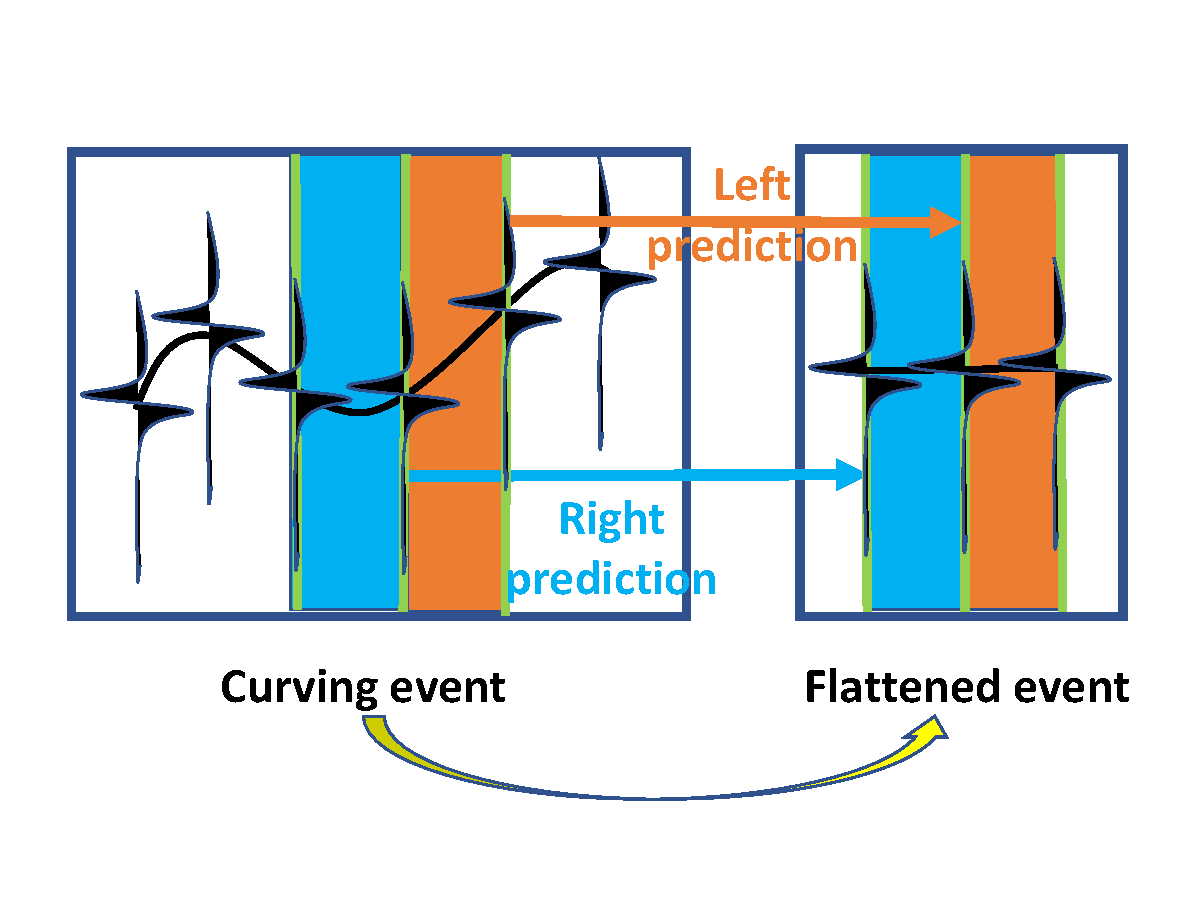
\includegraphics[width=0.32\columnwidth,height=0.32\columnwidth]{Fig/demo}
%  \caption{Demonsration of global orthogonalization.}
%   \label{fig:demo}
%\end{figure}

\begin{align}
\label{eq:ortho1}
\hat{\mathbf{n}} &= \mathbf{n}_0 - w\mathbf{s}_0, \\
\label{eq:ortho2}
\hat{\mathbf{s}} &= \mathbf{s}_0 + w\mathbf{s}_0.
\end{align}
In a local sense, the LOW can be define as:
      \begin{equation}
        \label{eq:eq2}
          w_m(t) = \frac{\displaystyle\sum_{i=t-m/2}^{t+m/2} s_0(i) n_0(i)}{\displaystyle\sum_{i=t-m/2}^{t+m/2} s_0^2(i)},
      \end{equation}
where $w_m(t)$ denotes the LOW for each temporal point $t$ with a local window length $m$. $s_0(t)$ and $n_0(t)$ here denote the initially estimated signal and noise for each point $t$.

In order to better control the locality and smoothness of LOW, we follow the local-attribute scheme introduced by \cite{fomel2007localattr}: %and first turn the orthogonalization problem into an optimization problem:
\begin{equation}
\label{eq:localortho}
\mathbf{w} = \arg\min_{\mathbf{\tilde{w}}} \parallel \mathbf{n}_0 - \mathbf{S}_0\mathbf{\tilde{w}}\parallel_2^2. %+ \mathbf{R}(\mathbf{w})
\end{equation}
Here, $\mathbf{w}$ is the LOW, $\mathbf{S}_0$ is a diagonal matrix composed of the initial estimated signal $\mathbf{s}_0$: $\mathbf{S}_0=diag(\mathbf{s}_0)$.
Then, we solve the least-squares problem \ref{eq:localortho} with the help of shaping regularization (a novel regularization framework for obtaining a faster convergence and a better control on the model behavior, originated from the seismic data processing community \cite{fomel2007shape}) using a local-smoothness constraint:
\begin{equation}
\label{eq:shape}
\mathbf{w} = [\lambda^2\mathbf{I} + \mathcal{T}(\mathbf{S}_0^T\mathbf{S}_0-\lambda^2\mathbf{I})]^{-1}\mathcal{T}\mathbf{S}_0^T\mathbf{n}_0,
\end{equation}
where $\mathcal{T}$ is a triangle smoothing operator and $\lambda$ is a scaling parameter set as $\lambda  = \Arrowvert\mathbf{S}_0^T\mathbf{S}_0\Arrowvert_2$ \cite{fomel2007localattr}. The triangle smoothing operator was introduced in detail in \cite{fomel2007shape}. It should be mentioned that solution of equation \ref{eq:localortho} corresponds to a regularized division (an element-wise division between two vectors can be treated as an inverse problem with some constraints in order to ensure the stability) between the two vectors $\mathbf{n}_0$ and $\mathbf{s}_0$ and it can be solved using any regularization approach, not limited to the shaping regularization strategy shown in equation \ref{eq:shape}. Thus it is fairly convenient to implement the local orthogonalization between initial signal and noise. A more detailed mathematical description about the local orthogonalization methodology can be found in \cite{yangkang2015ortho} and a demonstration about the physical meaning of orthogonalization can be found in the Appendix A in \cite{yangkang2015ortho}. 

\subsection{Local bandlimited orthogonalization}
\inputdir{.}

The basic principle of the proposed approach is to first apply a simple bandpass filter to the raw common shot gather in order to obtain an initial guess of primary reflections and ground-roll noise. Then we orthogonalize the initial guess for primary reflections and ground-roll noise to obtain a signal compensated primary reflection gather, and a signal-free ground-roll noise section. In order to make the local orthogonalization robust, we need first use a relative high LBF such that all the ground-roll noise is removed initially. This proposed workflow for attenuating ground-roll noise is termed \emph{local bandlimited orthogonalization}. The detailed workflow of the proposed approach is shown in Figure \ref{fig:flowchart}. As we can see, the total workflow of the proposed approach is fairly convenient to implement, because there are only two steps involved in the processing. First, we apply a conventional bandpass filter. Second, local signal-and-noise orthogonalization is applied. As we stated in the last section, the local signal-and-noise orthogonalization is no more than solving a regularized division problem (equations \ref{eq:eq2} and \ref{eq:localortho}). Thus, the proposed approach can be conveniently implemented by the industry. In the next section, we will use a typical dataset for demonstrating the effective performance of the proposed approach.

\plot{flowchart}{width=0.8\columnwidth}{Workflow of the proposed ground-roll noise attenuation approach based on local bandlimited orthogonalization.}

\section{Example}
The dataset that we use to demonstrate the effectiveness of our proposed denoising approach is \wen{an open-source dataset, which has been widely used in the geophysics community \cite{yilmaz1987,carson2006}.} \dlo{borrowed from  and }\wen{This data }is referred to as the OZ-25 dataset \cite{carson2006}. \wen{One can easily download it either from the Seismic Unix (SU) website ($http://www.cwp.mines.edu/cwpcodes/$) or from the Madagascar software website ($www.ahay.org$, \cite{mada2013}).} The raw data in common shot domain is shown in Figure \ref{fig:field}. \wen{The temporal sampling rate is 0.002s and the spatial sampling rate is 0.05km. The shot location is located at the middle of the receiver array, thus the shot record has a symmetric form. There are 81 traces (receivers) in the shot record and the offset ranges from -2km to 2km.} The OZ-25 dataset is a typical dataset suitable for testing the ground-roll noise attenuation performance because of several reasons. First,  there is a large amount of ground-roll noise contaminating this dataset. It is obvious that most of the primary reflections are covered by this coherent ground-roll noise. Secondly, the reflections are highly non-stationary. We can clearly see that the amplitudes of the reflections are variable in the range of the whole gather. 
%Because of the large amplitude range of primary reflections, it can be effectively used to test the primary reflections preservation properties of a certain denoising algorithm.   

\dlo{Figures \ref{fig:field-ortho-0} and \ref{fig:dif-ortho-0} show the denoised section and noise section using the proposed approach.} We locally orthogonalize the denoised section and noise section that come from the initial bandpass filtering using $fl=25$ Hz. The initial guess of the primary reflections and ground-roll noise are shown in Figures \ref{fig:field-1-0} and \ref{fig:dif-1-0}. \wen{Figures \ref{fig:field-ortho-0} and \ref{fig:dif-ortho-0} show the denoised section and noise section using the proposed approach.} The denoised data using the proposed approach shows excellent result, because most of the ground-roll noise has been removed, but no primary reflections energy is damaged. 

We also apply the widely used adaptive subtraction method to the field data and show its performance in Figures \ref{fig:field-3-0} and \ref{fig:dif-3-0}. Figures \ref{fig:field-3-0} and \ref{fig:dif-3-0} correspond to the denoised data and removed noise, respectively. It is obvious that there is some residual ground-roll noise remaining in the denoised data and that the noise section contains significant reflection energy, especially for the shallow part.

We zoom several parts from the denoised sections and noise sections and show them in Figures \ref{fig:zooma-1,zooma-2,zooma-ortho,zooma-3} and \ref{fig:zoomb-1,zoomb-2,zoomb-ortho,zoomb-3}. Figure \ref{fig:zooma-1,zooma-2,zooma-ortho,zooma-3} shows the zoomed denoised sections for the frame box A, as shown in Figures \ref{fig:field-1-0},\ref{fig:field-2-0}\dlo{ and }\wen{, }\ref{fig:field-ortho-0}, \wen{and \ref{fig:field-3-0},} respectively. We can see there is good primary reflection recovery using the proposed approach, by comparing Figures \ref{fig:zooma-1} and \ref{fig:zooma-ortho}. There is also an obvious decrease of noise using the proposed approach by comparing Figures \ref{fig:zooma-2} and \ref{fig:zooma-ortho}. \wen{It is more obvious that the adaptive subtraction method leaves some residual dipping ground-roll noise energy by comparing Figures \ref{fig:zooma-ortho} and \ref{fig:zooma-3}.}

Figure \ref{fig:zoomb-1,zoomb-2,zoomb-ortho,zoomb-3} shows the zoomed noise sections for frame box B, as shown in Figures \ref{fig:dif-1-0}, \ref{fig:dif-2-0},  \ref{fig:dif-ortho-0}, and \ref{fig:dif-3-0}, respectively. Please note that there is a decrease of primary reflections using the proposed approach, comparing Figures \ref{fig:zoomb-1} and \ref{fig:zoomb-ortho}, and there is an increase of noise removal using the proposed approach, comparing Figures \ref{fig:zoomb-2} and \ref{fig:zoomb-ortho}. \wen{The proposed approach and the adaptive subtraction method are very similar in this selected region. There is a slight amount of useful energy in Figure \ref{fig:zoomb-ortho} but hopefully not significant, considering the overall denoising performance. The ground-roll noise energy in Figure \ref{fig:zoomb-ortho}, however, is a bit stronger than that in Figure \ref{fig:zoomb-3}.} These observations indicate that compared with bandpass filtering with $fl=25$ Hz, the proposed approach preserves much more useful energy, and compared with bandpass filtering with $fl=10$ Hz, the proposed method removes much more ground-roll noise. \wen{Compared with the traditional adaptive subtraction method, the proposed approach can obtain a generally better performance}.

Figure \ref{fig:field-fs} shows a comparison of the average spectrum of all the traces for different data. The black solid line denotes the average spectrum of raw data. The green line corresponds to the proposed approach. The red line corresponds to the high-pass filtering with $fl=25$ Hz. The pink line corresponds to the high-pass filtering with $fl=10$ Hz. Blue corresponds to the adaptive subtraction method. We can see obviously that there is a removal of ground-roll noise spectrum from the black and yellow lines to the green line.  There is also a spectrum boost of the primary reflections between red and green. There exists several spectral notches for the blue spectrum, which indicates that there is still an overlap of reflections and ground-roll noise after applying the adaptive subtraction method.

\inputdir{field}

\plot{field}{width=.42\columnwidth}{Raw OZ-25 field data, borrowed from \cite{carson2006}.}

\multiplot{4}{field-1-0,dif-1-0,field-2-0,dif-2-0}{width=0.40\columnwidth}{(a) Bandpass filtered data (fl=25 Hz). (b) Difference section corresponding to (a). (c) Bandpass filtered data (fl=10 Hz). (d) Difference section corresponding to (c).}

\multiplot{4}{field-ortho-0,dif-ortho-0,field-3-0,dif-3-0}{width=0.40\columnwidth}{(a) Denoised data using the proposed approach. (b) Noise section corresponding to (a). (c) Denoised data using the adaptive subtraction approach. (d) Noise section corresponding to (c).}

\multiplot{4}{zooma-1,zooma-2,zooma-ortho,zooma-3}{width=0.35\columnwidth}{(a)-(d) Zoomed denoised section comparisons for frame box A (as shown in Figures \ref{fig:field-1-0},\ref{fig:field-2-0} , \ref{fig:field-ortho-0}, and \ref{fig:field-3-0}, respectively). Note the primary reflections recovery from (a) to (c) and the noise decrease from (b) to (c). There is obvious residual ground-roll noise existing in (d).}

\multiplot{4}{zoomb-1,zoomb-2,zoomb-ortho,zoomb-3}{width=0.35\columnwidth}{(a)-(d) Zoomed noise section comparisons for frame box B (as shown in Figures \ref{fig:dif-1-0},\ref{fig:dif-2-0}, \ref{fig:dif-ortho-0}, and \ref{fig:dif-3-0}, respectively). Note the decrease of primary reflections from (a) to (c) and the increase of noise removal from (b) to (c). (c) and (d) are very similar in this zoomed region.}

\plot{field-fs}{width=0.8\columnwidth}{Comparisons of the average spectrum of all the traces. The black line denotes the average spectrum of raw data. The green line corresponds to the proposed approach. The red line corresponds to $fl=25$ Hz. The pink line corresponds to $fl=10$ Hz. The blue line corresponds to the adaptive subtraction method. Note the removal of ground-roll noise spectrum from the black and pink lines to the green line, and the primary reflections spectrum boost from the red line to the green line. There exists several spectrum notches in the blue line, indicating a mixture of useful reflections and ground-roll noise after applying the adaptive subtraction method. }

\section{Conclusions}
We have proposed a novel local bandlimited  orthogonalization approach for removing highly non-stationary ground-roll noise, which can remove most ground-roll noise without harming the useful primary reflections. We orthogonalize the initial guess of primary reflections and ground-roll noise using local signal-and-noise orthogonalization. The initial guess of primary reflections and ground-roll noise are bandlimited data from a common bandpass filtering with a relatively high LBF such that all the ground-roll noise is removed during the initial guess. The proposed approach can solve the frequency-overlap problem when applying a simple bandpass filtering. The proposed approach can guarantee that the least amount of useful primary reflections is lost in the noise section. The procedure of the proposed approach is fairly convenient to implement because only a bandpass filtering and a regularized division between the initially denoised signal and initial noise are used. We have used an open-source field dataset to demonstrate the successful performance of the proposed approach in real data processing. 

\section{Acknowledgments}
We would like to thank Qun Luo, Shan Qu, Jiang Yuan, and two anonymous reviewers for constructive suggestions that improved the manuscript greatly. Yangkang Chen appreciates Sergey Fomel for the inspiring discussions about local orthogonalization. The paper is reproducible within the Madagascar open-source platform \cite{mada2013}. We are grateful to developers of the Madagascar software package for providing corresponding codes for testing the algorithms and preparing the figures. This work is partially supported by the Natural Science Fund of China (grant nos.:91330108, 41374121, and 61327013), the fundamental Research Funds for the Central Universities (grant no.: HIT.BRETIV.201314), the Program for New Century Excellent Talents in University (grant no.: NCET-11-0804), the China Postdoctoral Science Foundation (grant no.: 2014M561053), the Natural Science Foundation of Hebei Province (grant no.: F2013202254), and the Texas Consortium for Computational Seismology (TCCS).

\bibliographystyle{seg}
\bibliography{groll}







